\section{Durchführung}
\label{sec:Durchführung}

\subsection{Bestimmung der Zeitkonstanten}
\begin{figure}
    \centering
    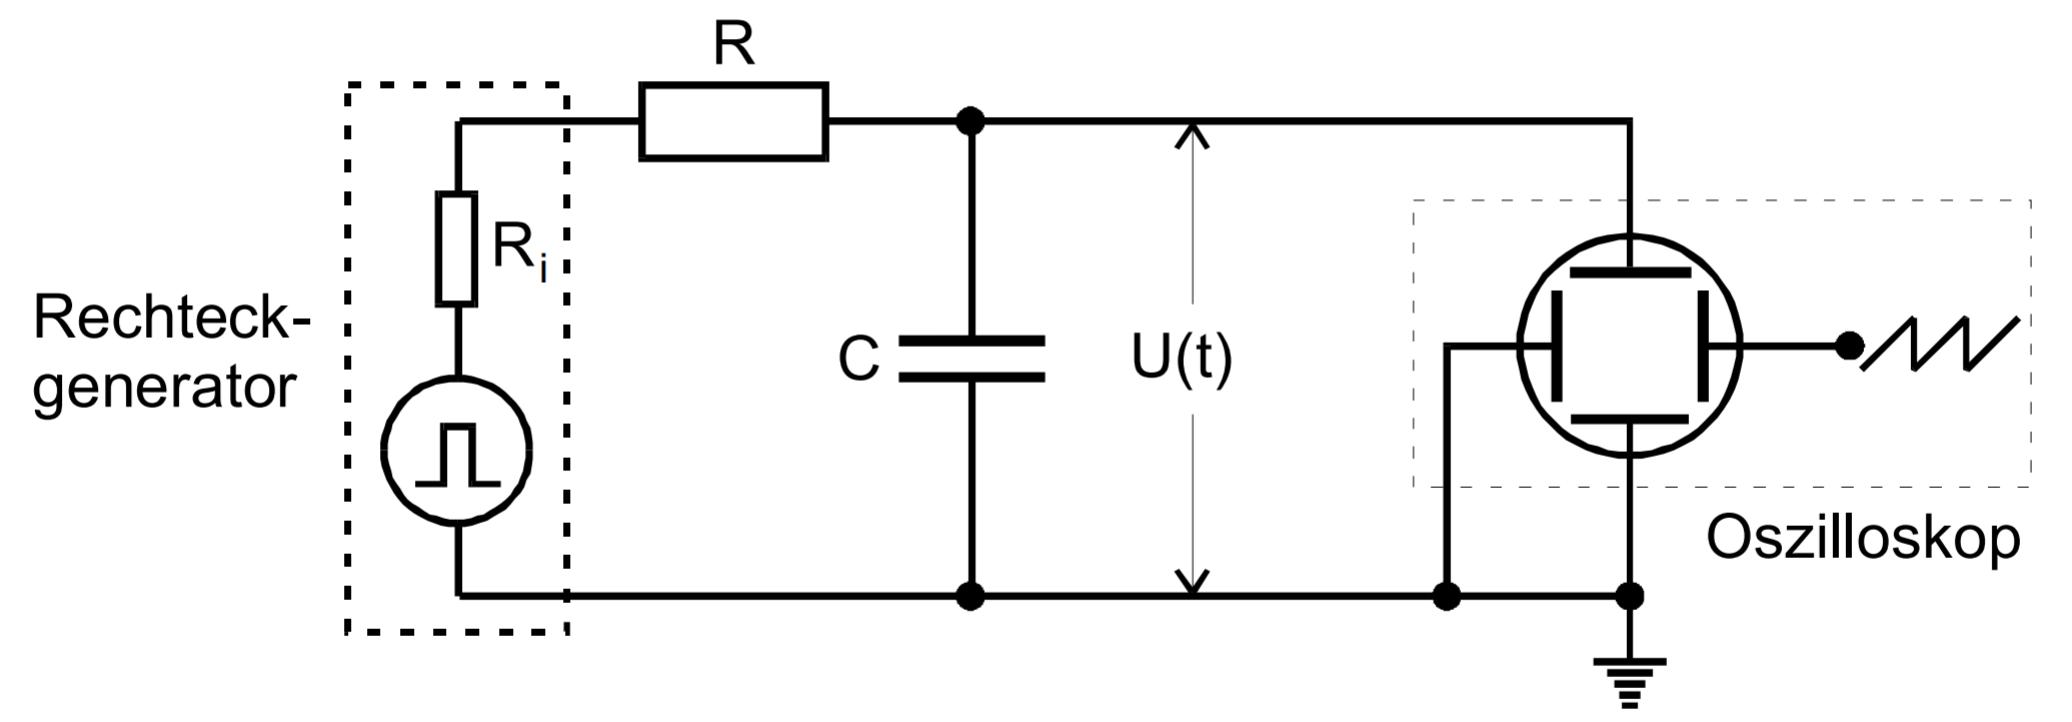
\includegraphics[width=\textwidth]{pictures/zeitkonstante.png}
    \caption{Schaltung zur Messung der Zeitkonstanten \cite{v353}.}
    \label{fig:zeitkonstante}
\end{figure}

Um die Zeitkonstante zu bestimmen, wird zunächst der RC-Kreis wie in Abbildung \ref{fig:zeitkonstante}
an ein Oszilloskop angeschlossen und mit einem Rechteckpuls $U_0 (t)$ angeregt.
Dabei ist der Widerstand $R$ und die Kapazität $C$ unbekannt.
Dann wird mit Hilfe des Triggers die Entladekurve der Kondensatorspannung $U_C (t)$ fixiert und
zu verschiedenen Zeiten $t$ notiert.

\subsection{Messung der Frequenzabhängigkeit und Phasenverschiebung}

\begin{figure}
    \centering
    \includegraphics[width=\textwidth]{pictures/Phasenverschiebung.png}
    \caption{Skizze einer Phasenverschiebung zweier Spannungen \cite{v353}.}
    \label{fig:phasenverschiebung}
\end{figure}

Nun soll die Frequenzabhängigkeit der Kondensatorspannung $U_C$ und die jeweilige
Phasenverschiebung zur Generatorspannung bestimmt werden.
Dafür wird die Anregungsfrequenz auf eine Sinusanregung umgestellt.
Es werden also jeweils die Frequenz $f$, die Phasenverschiebung $\phi$ und die Spannung $U_C$ notiert.
Die Phasenverschiebung wird am Oszilloskop einfach abgelesen, indem das Oszilloskop so eingestellt wird,
dass die beiden Symmetriepunkte der Generatorspannung und der Kondensatorspannung im Mittelpunkt sind.
Die Amplitude der Kondensatorspannung kann dann auch einfach abgelesen werden.
Die Frequenz wird einfach am Gerät eingestellt und notiert.

Aus dem Abstand der Nullstellen a und der Wellenlänge b berechnet sich die Phasenver-
schiebung über
\begin{equation} \label{eq:phase}
    \phi=\frac{a}{b} \cdot 2 \pi \, .
\end{equation}

\subsection{Dreiecksanregung eines RC-Kreises}

Am Schluss soll noch der RC-Kreis aus Abbildung \ref{fig:zeitkonstante} mit einer Dreiecksanregung angeregt werden
und dann für hohe Frequenzen beobachtet werden.
Dafür wird am Generator auf Dreiecksanregung gestellt und eine Frequenz von $f \geq 10 \si{\kilo\hertz}$ gewählt.